\documentclass[12pt,addpoints]{evalua}
\grado{2$^\circ$ de Secundaria}
\cicloescolar{2024-2025}
\materia{Ciencias y Tecnología: Física \normalfont \color{darkgray} \small \\[-0.2em] con adecuación curricular.}
\unidad{1}
\title{Examen de la Unidad}
\aprendizajes{\footnotesize%
\item Identifica problemas de la vida cotidiana y plantea soluciones.\\[-1.8em]
\item Conoce y caracteriza el pensamiento científico para plantearse y resolver problemas en la escuela y su cotidianidad.\\[-2em]
\item Valora la influencia del conocimiento científico y tecnológico en la sociedad actual.\\[-2em]
\item Identifica las unidades de medición que se ocupan en su entorno escolar, familiar y en su comunidad.\\[-2em]
\item Identifica cuáles son, cómo se definen y cuál es la simbología de las unidades básicas y derivadas del Sistema Internacional de Unidades.\\[-2em]
\item Realiza conversiones con los múltiplos y submúltiplos al referirse a una magnitud.\\[-2em]
\item Conoce los instrumentos de medición, materiales, sus propiedades y características.\\[-2em]
\item Relaciona e interpreta las teorías sobre estructura de la materia, a partir de los modelos atómicos y de partículas y los fenómenos que les dieron origen.\\[-2em]
\item Explora algunos avances recientes en la comprensión de la constitución de la materia y reconoce el proceso histórico de construcción de nuevas teorías.\\[-2em]
\item Experimenta e interpreta los modelos atómicos y de partículas al proponer hipótesis que expliquen los tres estados de la materia, sus propiedades físicas como la temperatura de fusión, ebullición, densidad, entre otros.\\[-2em]
\item Interpreta la temperatura y el equilibrio térmico con base en el modelo de partículas.\\[-2em]
% \item Describe problemas comunes de la vida cotidiana explicando cómo se procede para buscarles solución; conoce y caracteriza el pensamiento científico para plantearse y resolver problemas en la escuela y su cotidianidad.\\[-1.5em]
% \item Identifica las unidades de medición que se ocupan en su entorno escolar, familiar y en su comunidad.\\[-1.5em]
% \item Relaciona e interpreta las teorías sobre estructura de la materia, a partir de los modelos atómicos y de partículas y los fenómenos que les dieron origen.\\[-1.5em]
% \item Experimenta e interpreta los modelos atómicos y de partículas al proponer hipótesis que expliquen los tres estados de la materia, sus propiedades físicas como la temperatura de fusión, ebullición, densidad, entre otros.\\[-1.5em]
}
\author{Prof.: Julio César Melchor Pinto}
\begin{document}
% \begin{multicols}{2}
% \tableofcontents
% \end{multicols}\newpage
\begin{questions}
      \question[7]{Relaciona las magnitudes físicas fundamentales con su unidad de medida en el Sistema Internacional.

      \begin{multicols}{2}
            \begin{parts}\raggedleft
                  \part Longitud              \fillin[E][0.2in]
                  \part Temperatura           \fillin[B][0.2in]
                  \part Cantidad de sustancia \fillin[G][0.2in]
                  \part Corriente eléctrica   \fillin[D][0.2in]
                  \part Intensidad luminosa   \fillin[F][0.2in]
                  \part Tiempo                \fillin[A][0.2in]
                  \part Masa                  \fillin[C][0.2in]
            \end{parts}

            \columnbreak

            \begin{choices}
                  \choice Segundo
                  \choice Kelvin
                  \choice Kilogramo
                  \choice ampere
                  \choice Metro
                  \choice candela
                  \choice mol
            \end{choices}
      \end{multicols}
}

\question[10]{Selecciona la respuesta correcta:

      \begin{multicols}{2}
            \begin{parts}
                  \part La \fillin[Dilatación][2cm] ocurre cuando la temperatura de un sólido aumenta, haciendo que aumente su volumen.

                  \begin{choices}
                        \choice Dilatación
                        \choice	Evaporación
                        \choice	Fusión
                        \choice	Condensación
                  \end{choices}



                  \part Las siguientes son características de los gases, excepto:

                  \begin{choices}
                        \choice Se pueden comprimir.
                        \choice	Sus partículas están separadas en unas más simples con carga eléctrica.
                        \choice	No tienen forma definida.
                        \choice	No tienen volumen definido.
                  \end{choices}

                  \part ¿Qué fenómeno se observa cuando se empaña el vidrio de un auto?

                  \begin{choices}
                        \choice Solidificación
                        \choice	Fusión
                        \choice	Condensación
                        \choice	Evaporación
                  \end{choices}

                  \part ¿A qué se debe que el agua se evapore a $100^\circ$C al nivel del mar, pero a $70^\circ$C a 8,848 metros sobre el nivel del mar?

                  \begin{choices}
                        \choice A la presión
                        \choice	A la temperatura
                        \choice	A la altitud
                        \choice	Al tipo de agua
                  \end{choices}

                  \part Cuando se aplica alcohol a una herida y este se convierte en su forma gaseosa rápidamente, ¿qué cambio de estado ocurre?

                  \begin{choices}
                        \choice Ionización
                        \choice	Sublimación
                        \choice	Evaporación
                        \choice	Fusión
                  \end{choices}

                  \part Cuando un relámpago atraviesa la atmósfera, en su camino se forma plasma debido a la gran cantidad de energía que absorben las moléculas de la atmósfera. ¿Qué cambio de estado ocurre en esa situación?

                  \begin{choices}
                        \choice Deposición
                        \choice	Ionización
                        \choice	Fusión
                        \choice	Condensación
                  \end{choices}

                  \part ¿Cuál es el punto de fusión del agua?

                  \begin{choices}
                        \choice $10^\circ$C
                        \choice $8^\circ$C
                        \choice $5^\circ$C
                        \choice $0^\circ$C
                  \end{choices}

                  \part ¿Qué es la cohesión?

                  \begin{choices}
                        \choice La fuerza de repulsión que existe entre las partículas de una misma sustancia.
                        \choice	La fuerza de atracción que existe entre las partículas de una misma sustancia.
                        \choice	La fuerza de atracción que existe entre dos partículas con carga opuesta.
                        \choice	La fuerza de repulsión que existe entre dos partículas con la misma carga.
                  \end{choices}

                  \part Para comprender los estados de agregación de la materia se puede utilizar el modelo cinético de partículas, considerando...

                  \begin{choices}
                        \choice la cohesión y el tipo de sustancia que es.
                        \choice	la cohesión y la energía de las partículas.
                        \choice	la densidad y la temperatura.
                        \choice	la energía de las partículas y su temperatura.
                  \end{choices}

                  \part Son características de los sólidos, excepto:

                  \begin{choices}
                        \choice Sin forma definida
                        \choice	No se pueden comprimir
                        \choice	Cohesión entre sus partículas alta
                        \choice	Volumen definido
                  \end{choices}
            \end{parts}
      \end{multicols}
}

\newpage

\question[10]{Selecciona la respuesta correcta:

      \begin{multicols}{2}

            \begin{parts}
                  \part Según el modelo cinético de partículas, ¿cuál de las siguientes no es una característica de las partículas que conforman un gas?

                  \begin{choices}
                        \choice Son de gran tamaño.
                        \choice	Se comportan como esferas rígidas.
                        \choice	Su movimiento es aleatorio.
                        \choice	Se encuentran en constante movimiento.
                  \end{choices}

                  \part Son cambios de estado excepto:

                  \begin{choices}
                        \choice Ionización
                        \choice	Liofilización
                        \choice	Sublimación
                        \choice	Condensación
                  \end{choices}

                  \part ¿En cuál de los siguientes procesos ocurre fusión?

                  \begin{choices}
                        \choice Cuando la lluvia se transforma en nieve
                        \choice	Cuando se forman las nubes
                        \choice	Cuando se empaña un espejo
                        \choice	Cuando la roca se transforma en lava
                  \end{choices}

                  \part Según el modelo cinético de partículas, ¿cuál de las siguientes no es una característica de las partículas que conforman un gas?

                  \begin{choices}
                        \choice Se comportan como esferas rígidas.
                        \choice	Son de gran tamaño.
                        \choice	Se encuentran en constante movimiento.
                        \choice	Su movimiento es aleatorio.
                  \end{choices}

                  \part La energía cinética promedio de las partículas depende de...

                  \begin{choices}
                        \choice la presión.
                        \choice	la humedad.
                        \choice	la temperatura.
                        \choice	la cantidad de partículas.
                  \end{choices}

                  \part ¿Cómo es el movimiento de las partículas entre colisiones?

                  \begin{choices}
                        \choice En línea recta
                        \choice	En órbitas circulares
                        \choice	Errático
                        \choice	Uniformemente acelerado
                  \end{choices}

                  \part El volumen de un gas está conformado principalmente por...

                  \begin{choices}
                        \choice agua.
                        \choice	vacío.
                        \choice	partículas.
                        \choice	aire.
                  \end{choices}

                  \part ¿Qué implica que aumente la temperatura de un gas para las partículas que lo conforman?

                  \begin{choices}
                        \choice Aumenta su energía cinética.
                        \choice	Disminuye el número de colisiones entre partículas.
                        \choice	La cantidad de vacío disminuye.
                        \choice	Se mueven más lentamente.
                  \end{choices}


                  \part La energía cinética promedio de las partículas depende de...

                  \begin{choices}
                        \choice la presión.
                        \choice	la cantidad de partículas.
                        \choice	la humedad.
                        \choice	la temperatura.
                  \end{choices}

                  \part ¿Cómo es el movimiento de las partículas entre colisiones?

                  \begin{choices}
                        \choice Uniformemente acelerado
                        \choice	Errático
                        \choice	En línea recta
                        \choice	En órbitas circulares
                  \end{choices}
            \end{parts}
      \end{multicols}
}

\newpage

\question[10]{Elige la respuesta correcta.

      \begin{multicols}{2}
            \begin{parts}%\footnotesize%
                  \part Es el espacio que ocupa un objeto.

                  \begin{multicols}{2}
                        \begin{choices}
                              \choice Masa  \choice Densidad  \CorrectChoice Volumen  \choice Materia
                        \end{choices}
                  \end{multicols}

                  \part Es la cantidad de materia que posee un cuerpo.

                  \begin{multicols}{2}
                        \begin{choices}
                              \CorrectChoice Masa  \choice Densidad  \choice Volumen  \choice Materia
                        \end{choices}
                  \end{multicols}

                  \part  Es todo aquello que ocupa un lugar en espacio.

                  \begin{multicols}{2}
                        \begin{choices}
                              \choice Masa  \choice Densidad  \choice Volumen  \CorrectChoice Materia
                        \end{choices}
                  \end{multicols}

                  % \part La materia \dots

                  % \begin{choices}
                  %      \choice no se puede medir.  \choice es detectable con distintos medios.  \choice no se puede observar.  \choice no ocupa un lugar en el espacio.
                  % \end{choices}

                  \part Son materiales que permiten la conducción de calor y electricidad.

                  \begin{multicols}{2}
                        \begin{choices}
                              \choice  inorgánicos  \choice  metálicos  \choice  tóxicos  \choice  refractarios
                        \end{choices}
                  \end{multicols}

                  % \part Son propiedades de la materia:

                  % \begin{choices}
                  %      \choice aceleración y fuerza.  \choice distintos medios de propagación.  \choice emoción y sueño.  \choice forma, volumen, masa y compresibilidad.
                  % \end{choices}

                  %      \part ¿Qué es la materia?

                  %      \begin{choices}
                  %           \choice La capacidad que tiene un objeto para interactuar con otros \choice El producto de la aceleración por la masa \choice Todo lo que ocupa un lugar en el espacio \choice Todo lo que se puede detectar
                  %      \end{choices}

                  \part Son materiales derivados del petróleo y pueden ser moldeados para lograr distintos objetos.

                  \begin{multicols}{2}
                        \begin{choices}
                              \choice  refractarios  \choice  plásticos  \choice  textiles  \choice  metálicos.
                        \end{choices}
                  \end{multicols}
            \end{parts}
      \end{multicols}
}

\question[15]{Analiza las siguientes afirmaciones. Luego, escribe un V si es verdadero o una F si es falsa.

      % \begin{multicols}{3}
      \begin{parts}
            \part \fillin[V][2cm] En los gases, la fuerza de atracción es menor que la fuerza de atracción.
            \part \fillin[V][2cm] Si la temperatura de un gas es alta, la rapidez de sus partículas también lo es.
            \part \fillin[V][2cm] La presión de los gases se debe al impacto que ejercen las moléculas del gas sobre las paredes del recipiente que los contiene.
            \part \fillin[V][2cm] Los líquidos poseen menos energía cinética que los gases.
            \part \fillin[V][2cm] En estado sólido las partículas presentan mayor energía cinética que en estado líquido
            \part \fillin[V][2cm] La sublimación, fusión y evaporación se producen por absorción de calor
            \part \fillin[V][2cm] La temperatura se puede medir con un termómetro y comúnmente utilizamos una escala llamada Celsius
            \part \fillin[V][2cm] En estado líquido y gas las partículas ocupan todo el volumen disponible
            \part \fillin[V][2cm] Al meter agua en el congelador para obtener hielo se está produciendo un cambio llamado fusión
            \part \fillin[V][2cm] Al observar “humo” saliendo de la escarcha se presencia el cambio llamado sublimación
            \part \fillin[V][2cm] Las partículas en un cuerpo en estado gaseoso presentan escasa distancia entre ellas
            \part \fillin[V][2cm] En estado sólido la materia adopta la forma del recipiente que la contiene
            \part \fillin[V][2cm] El calor permite incrementar la energía cinética de las partículas
            \part \fillin[V][2cm] Al cambiar de estado, el agua mantiene constante la temperatura
            \part \fillin[V][2cm] Al hervir la tetera se observa un cambio de estado llamado evaporación
      \end{parts}
      % \end{multicols}
}

% 	\addcontentsline{toc}{section}{L8 Materiales y sus propiedades}
% \section*{L8 Materiales y sus propiedades}
\newpage

\question[9]{Selecciona la respuesta correcta:

      \begin{multicols}{3}
            \begin{parts}
                  \part Observa el diagrama y responde: ¿Qué estado de la materia tiene partículas con mayor energía cinética?
                  \begin{center}
                        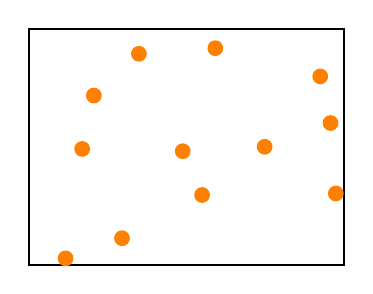
\begin{tikzpicture}
                              \draw[thick] (0,0) rectangle (4,3);
                              \foreach \x in {0.5,1.5,2.5,3.5} {
                                          \foreach \y in {0.5,1.5,2.5} {
                                                      \fill[orange] (\x + 0.5*rand, \y + 0.5*rand) circle (0.1);
                                                }
                                    }
                        \end{tikzpicture}
                  \end{center}


                  \begin{oneparchoices}
                        \choice Sólido
                        \choice Líquido \\
                        \CorrectChoice Gas
                        \choice Plasma
                  \end{oneparchoices}

                  \part Observa el diagrama y responde: ¿Qué estado de la materia tiene partículas con mayor energía cinética?
                  \begin{center}
                        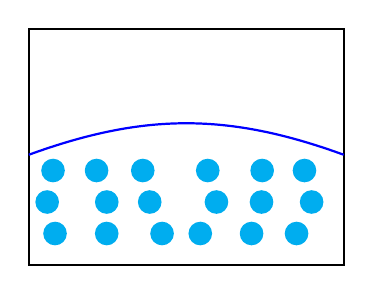
\begin{tikzpicture}
                              \draw[thick] (0,0) rectangle (4,3);
                              \draw[thick, blue] (0,1.4) to[out=20,in=160] (4,1.4);
                              \foreach \x in {0.4,1.0,1.6,2.2,2.8,3.4} {
                                          \foreach \y in {0.4,0.8,1.2} {
                                                      \fill[cyan] (\x+rand*0.2,\y) circle (0.15);
                                                }
                                    }
                        \end{tikzpicture}
                  \end{center}

                  \begin{oneparchoices}
                        \choice Sólido
                        \CorrectChoice Líquido \\
                        \choice Gas
                        \choice Plasma
                  \end{oneparchoices}

                  \part Observa el diagrama y responde: ¿Qué estado de la materia tiene partículas con mayor energía cinética?
                  \begin{center}
                        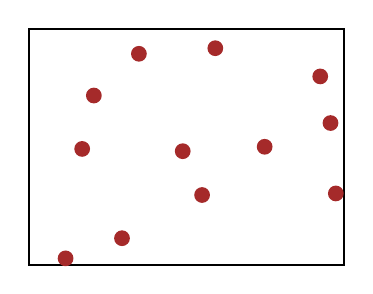
\begin{tikzpicture}
                              \draw[thick] (0,0) rectangle (4,3);
                              \foreach \x in {0.5,1.5,2.5,3.5} {
                                          \foreach \y in {0.5,1.5,2.5} {
                                                      \fill[Brown] (\x + 0.5*rand, \y + 0.5*rand) circle (0.1);
                                                }
                                    }
                        \end{tikzpicture}
                  \end{center}

                  \begin{oneparchoices}
                        \choice Sólido
                        \choice Líquido \\
                        \CorrectChoice Gas
                        \choice Plasma
                  \end{oneparchoices}

                  \part Observa el diagrama y responde: ¿Qué estado de la materia tiene partículas con mayor energía cinética?
                  \begin{center}
                        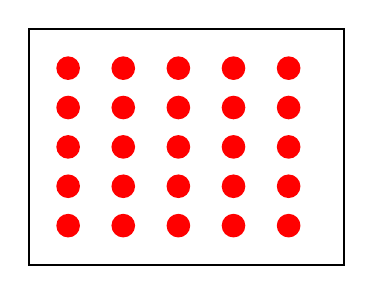
\begin{tikzpicture}
                              \draw[thick] (0,0) rectangle (4,3);
                              \foreach \x in {0.5,1.2,1.9,2.6,3.3} {
                                          \foreach \y in {0.5,1.0,1.5,2.0,2.5} {
                                                      \fill[Red] (\x,\y) circle (0.15);
                                                }
                                    }
                        \end{tikzpicture}
                  \end{center}

                  \begin{oneparchoices}
                        \CorrectChoice Sólido
                        \choice Líquido \\
                        \choice Gas
                        \choice Plasma
                  \end{oneparchoices}


                  \part Observa el diagrama y responde: ¿Qué estado de la materia tiene partículas con mayor energía cinética?
                  \begin{center}
                        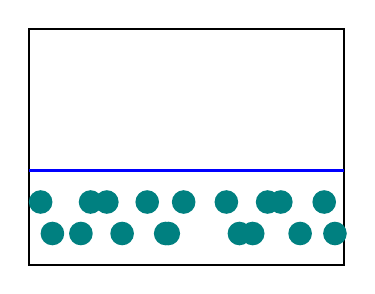
\begin{tikzpicture}
                              \draw[thick] (0,0) rectangle (4,3);
                              \draw[thick, blue] (0,1.2) -- (4,1.2);
                              \foreach \x in {0.4,0.8,1.2,1.6,2.0,2.4,2.8,3.2,3.6} {
                                          \foreach \y in {0.4,0.8} {
                                                      \fill[teal] (\x+rand*0.3,\y) circle (0.15);
                                                }
                                    }
                        \end{tikzpicture}
                  \end{center}

                  \begin{oneparchoices}
                        \choice Sólido
                        \CorrectChoice Líquido \\
                        \choice Gas
                        \choice Plasma
                  \end{oneparchoices}

                  \part Observa el diagrama y responde: ¿Qué estado de la materia tiene partículas con mayor energía cinética?
                  \begin{center}
                        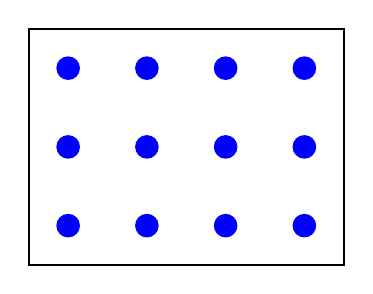
\begin{tikzpicture}
                              \draw[thick] (0,0) rectangle (4,3);
                              \foreach \x in {0.5,1.5,2.5,3.5} {
                                          \foreach \y in {0.5,1.5,2.5} {
                                                      \fill[blue] (\x,\y) circle (0.15);
                                                }
                                    }
                        \end{tikzpicture}
                  \end{center}

                  \begin{oneparchoices}
                        \CorrectChoice Sólido
                        \choice Líquido \\
                        \choice Gas
                        \choice Plasma
                  \end{oneparchoices}

                  \part Observa el diagrama y responde: ¿Qué estado de la materia tiene partículas con mayor energía cinética?
                  \begin{center}
                        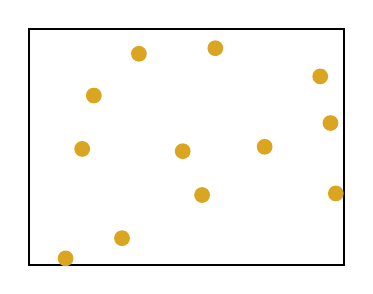
\begin{tikzpicture}
                              \draw[thick] (0,0) rectangle (4,3);
                              \foreach \x in {0.5,1.5,2.5,3.5} {
                                          \foreach \y in {0.5,1.5,2.5} {
                                                      \fill[Goldenrod] (\x + 0.5*rand, \y + 0.5*rand) circle (0.1);
                                                }
                                    }
                        \end{tikzpicture}
                  \end{center}

                  \begin{oneparchoices}
                        \choice Sólido
                        \choice Líquido \\
                        \CorrectChoice Gas
                        \choice Plasma
                  \end{oneparchoices}

                  \part Observa el diagrama y responde: ¿Qué estado de la materia tiene partículas con mayor energía cinética?
                  \begin{center}
                        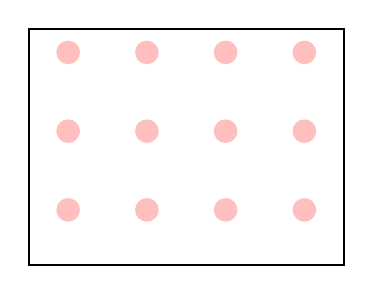
\begin{tikzpicture}
                              % Dibujo del matraz
                              \draw[thick] (0,0) rectangle (4,3);
                              % Partículas escalonadas
                              \foreach \x in {0.5,1.5,2.5,3.5} {
                                          \foreach \y in {0.7,1.7,2.7} {
                                                      \fill[pink] (\x,\y) circle (0.15);
                                                }
                                    }
                        \end{tikzpicture}
                  \end{center}

                  \begin{oneparchoices}
                        \CorrectChoice Sólido
                        \choice Líquido \\
                        \choice Gas
                        \choice Plasma
                  \end{oneparchoices}

                  \part Observa el diagrama y responde: ¿Qué estado de la materia tiene partículas con mayor energía cinética?
                  \begin{center}
                        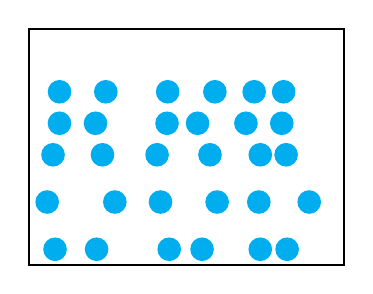
\begin{tikzpicture}
                              % Dibujo del matraz
                              \draw[thick] (0,0) rectangle (4,3);
                              % Partículas distribuidas aleatoriamente
                              \foreach \x in {0.4,1.0,1.6,2.2,2.8,3.4} {
                                          \foreach \y in {0.2,0.8,1.4,1.8,2.2} {
                                                      \fill[cyan] (\x + rand*0.2,\y) circle (0.15);
                                                }
                                    }
                        \end{tikzpicture}
                  \end{center}

                  \begin{oneparchoices}
                        \choice Sólido
                        \CorrectChoice Líquido \\
                        \choice Gas
                        \choice Plasma
                  \end{oneparchoices}
            \end{parts}
      \end{multicols}
}

\newpage

\question[15]{Relaciona los conceptos de la columna izquierda con su descripción en la columna derecha:

      \begin{multicols}{2}
            \begin{parts}\raggedleft
                  \part Cambio de sólido a líquido. 											\fillin[][0.5cm]
                  \part Estado con partículas cercanas y organizadas. 						\fillin[][0.5cm]
                  \part Cambio de líquido a gas. 												\fillin[][0.5cm]
                  \part Propiedad de movimiento de las partículas. 							\fillin[][0.5cm]
                  \part Partículas en estado ionizado. 										\fillin[][0.5cm]
                  \part Cambio directo de sólido a gas. 										\fillin[][0.5cm]
                  \part Estado con partículas lejanas y desordenadas. 						\fillin[][0.5cm]
                  \part Movimiento de partículas de mayor concentración a menor. 				\fillin[][0.5cm]
                  \part Cambio de gas a líquido. 												\fillin[][0.5cm]
                  \part Estado fluido sin forma fija pero con volumen definido. 				\fillin[][0.5cm]
                  \part Relación entre masa y volumen. 										\fillin[][0.5cm]
                  \part Cambio en el que no se altera la composición. 						\fillin[][0.5cm]
                  \part Temperatura en la que hierve una sustancia. 							\fillin[][0.5cm]
                  \part Proceso de cambio líquido a gas a temperatura ambiente. 				\fillin[][0.5cm]
                  \part Cambio de gas a líquido. 												\fillin[][0.5cm]
            \end{parts}

            \columnbreak

            \begin{choices}
                  \choice Condensación.
                  \choice Fusión.
                  \choice Vaporización.
                  \choice Energía Cinética.
                  \choice Difusión.
                  \choice Líquido.
                  \choice Gas.
                  \choice Plasma.
                  \choice Sublimación.
                  \choice Punto de ebullición.
                  \choice Cambio físico.
                  \choice Evaporación.
                  \choice Condensación.
                  \choice Sólido.
                  \choice Densidad.
            \end{choices}
      \end{multicols}
}

\question[14]{Señala si los siguientes procesos son \textit{físicos} o \textit{químicos}.

      \begin{multicols}{3}
            \begin{parts}
                  \part Romper una hoja de papel.

                  \begin{oneparchoices}
                        \CorrectChoice Físico \choice Químico
                  \end{oneparchoices}

                  \part Digerir y absorber los alimentos.


                  \begin{oneparchoices}
                        \choice Físico \CorrectChoice Químico
                  \end{oneparchoices}

                  \part Derretir una vela.


                  \begin{oneparchoices}
                        \CorrectChoice Físico \choice Químico
                  \end{oneparchoices}

                  \part Encender fuegos artificiales.


                  \begin{oneparchoices}
                        \choice Físico \CorrectChoice Químico
                  \end{oneparchoices}

                  \part Hornear un pastel de vainilla.


                  \begin{oneparchoices}
                        \choice Físico \CorrectChoice Químico
                  \end{oneparchoices}

                  \part Apretar una lata de aluminio.


                  \begin{oneparchoices}
                        \CorrectChoice Físico \choice Químico
                  \end{oneparchoices}

                  \part Derretir un cubo de hielo.


                  \begin{oneparchoices}
                        \CorrectChoice Físico \choice Químico
                  \end{oneparchoices}

                  \part Cocinar un huevo estrellado.

                  \begin{oneparchoices}
                        \choice Físico \CorrectChoice Químico
                  \end{oneparchoices}

                  

                  \part Hundir un clavo en una pared.

                  \begin{oneparchoices}
                        \CorrectChoice Físico \choice Químico
                  \end{oneparchoices}

                  \part Machacar una piedra.
      
                  \begin{oneparchoices}
                        \CorrectChoice Físico \choice Químico
                  \end{oneparchoices}

                  

                  \part Mezclar agua con aceite.

                  \begin{oneparchoices}
                        \CorrectChoice Físico \choice Químico
                  \end{oneparchoices}

                  \part Mojar un papel.
            
                  \begin{oneparchoices}
                        \CorrectChoice Físico \choice Químico
                  \end{oneparchoices}

                  \part Fermentación de la uva para hacer vino.

                  \begin{oneparchoices}
                        \choice Físico \CorrectChoice Químico
                  \end{oneparchoices}

                  \part Corrosión de una estatua de bronce:.
      
                  \begin{oneparchoices}
                        \choice Físico \CorrectChoice Químico
                  \end{oneparchoices}
            \end{parts}
      \end{multicols}
}

\newpage 

\question[10]{Selecciona la respuesta correcta:
      \begin{multicols}{2}
            \begin{parts}
                  % \part ¿Qué se necesita tomar en cuenta para poder aplicar el modelo cinético de partículas a los líquidos y los gases?

                  % \begin{choices}
                  % 	\choice El estado de agregación.
                  % 	\choice	La cantidad de materia presente.
                  % 	\choice	La forma del recipiente que los contiene.
                  % 	\choice	Las fuerzas de atracción entre partículas.
                  % \end{choices}
                  \part ¿Cuál de los siguientes es la abreviatura de kilogramo

                  \begin{choices}
                        \choice ml
                        \choice cc
                        \choice g
                        \choice kg
                  \end{choices}

                
                  \part El término "energía cinética" se refiere a:
          
                  \begin{choices}
                        \choice La energía almacenada en las partículas
                        \choice La energía del movimiento de las partículas
                        \choice La energía potencial de las partículas
                        \choice La energía total de un objeto en reposo
                  \end{choices}

                  \part ¿Qué estado de la materia tiene partículas muy juntas y organizadas?
               
                  \begin{choices}
                        \choice Sólido
                        \choice Líquido
                        \choice Gas
                        \choice Plasma
                  \end{choices}

                  \part ¿Cómo se llama el proceso mediante el cual un sólido pasa directamente a gas?
                 
                  \begin{choices}
                        \choice Condensación
                        \choice Sublimación
                        \choice Evaporación
                        \choice Fusión
                  \end{choices}

                  \part ¿Qué estado de agregación se caracteriza por tener volumen definido, pero toma la forma del recipiente que lo contiene?

                  \begin{choices}
                        \choice Líquido
                        \choice	Sólido
                        \choice	Plasma
                        \choice	Gas
                  \end{choices}

                  \part ¿Qué propiedad es característica del estado gaseoso?
           
                  \begin{choices}
                        \choice Volumen definido
                        \choice Forma fija
                        \choice Partículas en movimiento desordenado
                        \choice Rigidez estructural
                  \end{choices}

                  \part ¿Qué sucede con las partículas de una sustancia al aumentar su temperatura?
                 
                  \begin{choices}
                        \choice Se acercan más entre sí
                        \choice Pierden energía
                        \choice Aumentan su energía cinética
                        \choice Se transforman en sólido
                  \end{choices}


                  \part ¿Qué se necesita tomar en cuenta para poder aplicar el modelo cinético de partículas a los líquidos y los gases?

                  \begin{choices}
                        \choice El estado de agregación.
                        \choice	La cantidad de materia presente.
                        \choice	La forma del recipiente que los contiene.
                        \choice	Las fuerzas de atracción entre partículas.
                  \end{choices}


                  \part El agua en forma de vapor se encuentra en el estado:
                
                  \begin{choices}
                        \choice Sólido
                        \choice Líquido
                        \choice Gas
                        \choice Plasma
                  \end{choices}

                  \part  ¿Cuál de los siguientes es la abreviatura de mililitros?

                  \begin{choices}
                        \choice g
                        \choice kg
                        \choice ml
                        \choice mg
                  \end{choices}

                  

            \end{parts}
      \end{multicols}
}
\end{questions}
\end{document}